\documentclass[a4paper, 12pt]{article}
\usepackage[top=1.5cm, bottom=2.2cm, left=2cm, right=2cm]{geometry}
\usepackage[utf8]{inputenc}
\usepackage{graphicx, caption}
\usepackage{float}
\usepackage{amsmath, amsfonts, amssymb, esint}
\usepackage{hyperref}
\usepackage{multicol}
\usepackage{color}
\usepackage{wallpaper}
\usepackage{array}

\CenterWallPaper{1}{./img/background.png}

\hypersetup{
    colorlinks=true,
    linkcolor=blue,
    filecolor=magenta,      
    urlcolor=cyan,
}

\newcolumntype{M}[1]{>{\centering\arraybackslash}m{#1}}

\definecolor{red}{rgb}{1,0,0}
\newcommand{\red}[1]{\textcolor{red}{#1}}

\begin{document}
    \begin{figure}
        \centering
        \href{https://ligaolimpicadeastronomia.com.br/}{
\includegraphics[scale=0.6]{./img/logos.png}}
    \end{figure}
    \begin{center}
        \begin{large}
            \textbf{Simulado 2 -- Intensivão para a OBA}
            \linebreak \red{Gabarito}
        \end{large}
        \end{center}
    \begin{flushright}
        Material elaborado por \textbf{Giulia Nóbrega} e \textbf{Iago Mendes}.
    \end{flushright}
    \red{Observação: \begin{itemize}
        \item As alternativas das perguntas deste gabarito não estão na mesma ordem do simulado.
    \end{itemize}}

    \section*{Questões de Astronomia}
        \begin{flushleft} \begin{itemize}
            \item \textbf{Questão 1) (1 ponto)} A imagem abaixo traz 2 constelações muito famosas. A partir da imagem, responda o que se pede:
                \begin{figure}[H]
                    \centering
                    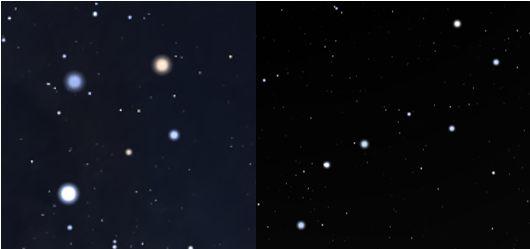
\includegraphics[scale=0.5]{./img/1.png}
                \end{figure}
                \begin{itemize}
                    \item \textbf{Pergunta 1a) (1 ponto) (0,5 ponto cada acerto)} Identifique quais são as constelações na imagem.
                    \begin{center} \begin{tabular}
                    {
                        |M{0.20\textwidth}|M{0.10\textwidth}|M{0.10\textwidth}|M{0.10\textwidth}|M{0.10\textwidth}|
                    }
                        \hline
                        $\quad$ & Centauro & Cruzeiro do Sul & Cisne & Ursa Maior \\ \hline
                        Constelação da esquerda & $\quad$ & \red{X} & $\quad$ & $\quad$ \\ \hline
                        Constelação da direita & $\quad$ & $\quad$ & $\quad$ & \red{X} \\ \hline
                    \end{tabular} \end{center}
                \end{itemize}
            
            \item \textbf{Questão 2) (1 ponto)} Abaixo temos descrições de diversos corpos celestes. Identifique-os:
                \begin{itemize}
                    \item \textbf{Pergunta 2a) (0,25 ponto)} Este corpo constantemente se afasta da Terra. Possui sempre a mesma face voltada para a Terra, ou seja, é bloqueado por marés.
                        \begin{itemize}
                            \item[$(\red{X})$] Lua
                            \item[$(\quad)$] Sol
                            \item[$(\quad)$] Vênus
                            \item[$(\quad)$] Marte
                        \end{itemize}
                    \item \textbf{Pergunta 2b) (0,25 ponto)} Orbita um planeta que possui apenas dois satélites naturais, sendo sua órbita a de menor raio. Com o passar do tempo se aproxima cada vez mais de seu planeta, o que indica que futuramente será despedaçado devido à força gravitacional exercida pelo corpo maior.
                        \begin{itemize}
                            \item[$(\red{X})$] Fobos
                            \item[$(\quad)$] Deimos
                            \item[$(\quad)$] Ceres
                            \item[$(\quad)$] Lua
                        \end{itemize}
                    \item \textbf{Pergunta 3c) (0,5 ponto)} É azulado e possui anéis. Demora aproximadamente 84 anos para completar sua translação. Possui 27 satélites naturais, sendo os principais Miranda, Ariel, Umbriel, Titânia e Oberon. É o menos massivo dos planetas gigantes.
                        \begin{itemize}
                            \item[$(\red{X})$] Urano
                            \item[$(\quad)$] Júpiter
                            \item[$(\quad)$] Saturno
                            \item[$(\quad)$] Netuno
                        \end{itemize}
                \end{itemize}

            \item \textbf{Questão 3) (1 ponto)} Na astronomia muitas vezes é útil estimar a altura de um objeto celeste. Como trabalhamos com corpos muito distantes de nós, a altura que medimos não é um comprimento, e sim um ângulo. Um dos objetos mais famosos utilizados para auxiliar esse cálculo é o sextante, que inclusive dá nome a uma constelação do hemisfério sul. Um aluno da OBA decide tentar fazer o mesmo, porém como não tem um sextante resolve improvisar. Ele finca uma vara de madeira de $1 \, m$ no chão e percebe que a sombra do objeto possui $1,2 \, m$. \linebreak \linebreak Dados: \linebreak $\tan(30^{\circ}) \approx 0,58$ \linebreak $\tan(60^{\circ}) \approx 1,73$ \linebreak \linebreak Dica: \linebreak Lembre-se que para $x$ entre $0^{\circ}$ e $90^{\circ}$ a função $\tan(x)$ é estritamente crescente.
                \begin{itemize}
                    \item \textbf{Pergunta 3) (1 ponto)} Qual é aproximadamente a altura do Sol?
                        \red{\begin{itemize}
                            \item Chamando a altura de Sol de $h$ e usando o cenário descrito, podemos calcular o $\tan h$:
                                \begin{equation*}
                                    \tan h = \frac{1}{1,2} \approx 0,83
                                \end{equation*}
                            \item Usando os valores das tangentes de $30^{\circ}$ e $60^{\circ}$ -- e lembrando que $\tan (40^{\circ}) = 1$ --, deduzimos que $30^{\circ} \leq h \leq 45^{\circ}$. Portanto, a única alternativa válida é $40^{\circ}$
                        \end{itemize}}
                        \begin{itemize}
                            \item[$(\quad)$] $10^{\circ}$
                            \item[$(\red{X})$] $40^{\circ}$
                            \item[$(\quad)$] $60^{\circ}$
                            \item[$(\quad)$] $80^{\circ}$
                        \end{itemize}
                \end{itemize}

            \item \textbf{Questão 4) (1 ponto)} Uma das missões da astronomia é determinar a distância de corpos luminosos até nós. Para isso, é muito comum estudar como a luz destes objetos se comporta. A prática mais comum é medir o fluxo de energia de tal corpo na Terra e assim, sabendo sua luminosidade, estimar sua distância. O espaço, no entanto, não é vazio, e a poeira interestelar nele presente absorve parte da radiação emitida, diminuindo a intensidade luminosa que captamos na Terra. Uma das equações mais utilizadas por nós para analisar esse efeito é a seguinte: $F'=F e^{-nVA}$ onde $F'$ é o fluxo captado na Terra, $F$ é o fluxo que seria captado se não houvesse extinção, $e$ é o número de Euler, $V$ é o volume da nuvem de poeira e $A$ é a área de seção transversal de um grão de poeira. Utilizando seus conhecimentos sobre análise dimensional, responda:
                \begin{itemize}
                    \item \textbf{Pergunta 4a) (0,5 ponto)} O que $n$ pode representar?
                        \red{\begin{itemize}
                            \item Considere $\alpha=-nVA$ como sendo o expoente da equação passada. Para que $\alpha$ seja adimensional, temos a seguinte unidade para $n$:
                                \begin{equation*} \begin{gathered}
                                    .[n] \cdot [V] \cdot [A] = 1 \quad \therefore \quad [n]=\frac{1}{[V] \cdot [A]}=\frac{1}{m^3 \cdot m^2} \\
                                    \therefore \quad [n] = \frac{1}{m^5} = m^{-5}
                                \end{gathered} \end{equation*}
                            \item Como a unidade de $n$ envolve somente comprimento, podemos eliminar as 2 últimas alternativas (considerando a ordem neste gabarito). Para que a resposta fosse a primeira alternativa, $[n]$ deveria ser $m$. Portanto, ficamos com a segunda alternativa.
                            \item Uma maneira mais fácil de entender o que $n$ representa seria dizer o número de partículas por volume de poeira interestelar por área de um grão de poeira, ou seja, uma densidade numérica.
                        \end{itemize}}
                        \begin{itemize}
                            \item[$(\quad)$] A distância percorrida pela luz dentro da nuvem de poeira
                            \item[$(\red{X})$] A densidade numérica de partículas na nuvem
                            \item[$(\quad)$] O tempo que a luz demora para percorrer a nuvem de poeira
                            \item[$(\quad)$] A massa da nuvem de poeira
                        \end{itemize}
                    \item \textbf{Pergunta 4b) (0,5 ponto)} O que aconteceria com F' se subitamente todos os grãos de poeira da nuvem dobrassem de tamanho?
                        \red{\begin{itemize}
                            \item Se os grãos de poeira aumentarem de tamanho, $A$ aumentará. Como $\alpha \propto - A$, o expoente de $e$ vai diminuir.
                            \item Além disso, pela equação dada, temos a seguinte proporção:
                                \begin{equation*}
                                    F' \propto e^\alpha
                                \end{equation*}
                            \item Portanto, $F'$ diminuirá.
                        \end{itemize}}
                        \begin{itemize}
                            \item[$(\quad)$] O expoente de $e$ vai aumentar e consequentemente $F'$ aumentará
                            \item[$(\quad)$] O expoente de $e$ vai aumentar e consequentemente $F'$ diminuirá
                            \item[$(\quad)$] O expoente de $e$ vai diminuir e consequentemente $F'$ aumentará
                            \item[$(\red{X})$] O expoente de $e$ vai diminuir e consequentemente $F'$ diminuirá
                        \end{itemize}
                \end{itemize}

            \item \textbf{Questão 5) (1 ponto)} Imagine que descobrimos um novo sistema planetário orbitando uma estrela muito distante. Essa estrela tem uma característica muito curiosa: sua densidade é igual a do Sol! A partir de diversas observações, astrônomos também descobriram que essa estrela é muito massiva, tendo uma massa de aproximadamente 1.000 vezes a massa do Sol (isso não seria possível na vida real, mas para o exercício vamos considerar que é!). \linebreak \linebreak Dados: \linebreak Massa do Sol $\approx 2 \cdot 10^{30} \, kg$ \linebreak Raio do Sol $\approx 7 \cdot 10^{8} \, m$ \linebreak $1 \, UA \approx 1,5 \cdot 10^{11} \, m$ \linebreak $\pi \approx 3$
                \begin{itemize}
                    \item \textbf{Pergunta 5a) (0,5 ponto)} Qual o volume dessa estrela?
                        \red{\begin{itemize}
                            \item Primeiramente, vamos relembrar da equação da densidade para esferas:
                                \begin{equation*}
                                    \rho = \frac{M}{V}=\frac{3M}{4\pi R^3}
                                \end{equation*}
                            \item Como a densidade das estrelas mencionadas no enunciado são iguais, temos:
                                \begin{equation*} \begin{gathered}
                                    \rho = \rho_{Sol} \quad \therefore \quad \frac{M}{V}=\frac{3M_{Sol}}{4\pi R_{Sol}^3} \\
                                    \therefore \quad V =\frac{4\pi MR_ {Sol}^3}{3M_{Sol}}=\frac{4 \pi 10^3 M_{Sol} R_{Sol}^3}{M_{Sol}}=\frac{4\cdot 3 \cdot 10^3 \cdot \left(7 \cdot 10^8\right)^3}{3} \approx 1,4 \cdot 10^{30} \, m^3
                                \end{gathered} \end{equation*}
                        \end{itemize}}
                        \begin{itemize}
                            \item[$(\quad)$] $\approx 5,2 \cdot 10^{25} \, m^3$
                            \item[$(\red{X})$] $\approx 1,4 \cdot 10^{30} \, m^3$
                            \item[$(\quad)$] $\approx 8,2 \cdot 10^{35} \, m^3$
                            \item[$(\quad)$] $\approx 3,4 \cdot 10^{40} \, m^3$
                        \end{itemize}
                    \item \textbf{Pergunta 5b) (0,5 ponto)} Se medirmos o raio desta estrela usando a distância da Terra ao Sol como unidade, qual será aproximadamente o resultado obtido?
                        \red{\begin{itemize}
                            \item Usando a mesma estratégia da pergunta anterior, temos:
                                \begin{equation*} \begin{gathered}
                                    V=10^3 \cdot V_{Sol} \quad \therefore \quad \frac{4\pi R^3}{3}=10^3 \cdot \frac{4 \pi R_{Sol}^3}{3}\\
                                    \therefore \quad R=10 \cdot R_{Sol} =10 \cdot 7 \cdot 10^8 = 7 \cdot 10^9 \, m
                                \end{gathered} \end{equation*}
                            \item Colocando em unidades astronômicas, temos:
                                \begin{equation*}
                                    V=\frac{7 \cdot 10^9}{1,5 \cdot 10^{11}} \approx 0,05 \, UA
                                \end{equation*}
                        \end{itemize}}
                        \begin{itemize}
                            \item[$(\red{X})$] $\approx 0,05 \, UA$
                            \item[$(\quad)$] $\approx 0,5 \, UA$
                            \item[$(\quad)$] $\approx 5 \, UA$
                            \item[$(\quad)$] $\approx 50 \, UA$
                        \end{itemize}
                \end{itemize}

            \item \textbf{Questão 6) (1 ponto)} Chamamos de quadratura o evento em que 2 corpos celestes formam um ângulo reto entre si, tendo um terceiro corpo como referência. Se tomarmos o Sol como centro, por exemplo, teremos dois planetas em quadratura quando o ângulo planeta1-Sol-planeta 2 for 90º. Para este exercício assuma que todos os planetas possuem órbitas circulares e tome o Sol como centro de qualquer quadratura mencionada. \linebreak \linebreak Dados: \linebreak Raio da órbita de Mercúrio: $0,4 \, UA$ \linebreak Raio da órbita de Vênus: $0,7 \, UA$ \linebreak Raio da órbita de Marte: $1,5 \, UA$ \linebreak Raio da órbita de Júpiter: $2,8 \, UA$
                \begin{itemize}
                    \item \textbf{Pergunta 6a) (0,5 ponto)} As distâncias da Terra a Mercúrio e a Vênus em uma quadratura são respectivamente:
                        \red{\begin{itemize}
                            \item Em uma quadratura, como o ângulo com vértice no Sol é reto, podemos aplicar o teorema de Pitágoras. Para planetas inferiores (Mercúrio e Vênus), temos o seguinte:
                                \begin{equation*}
                                    d^2=1^2+r^2 \quad \therefore \quad d=\sqrt{1+r^2}
                                \end{equation*}
                                em que $r$ é o raio orbital do planeta inferior e $d$ é a distância que queremos calcular.
                            \item Fazendo o cálculo para Mercúrio, temos:
                                \begin{equation*}
                                    d_m=\sqrt{1+0,4^2}=\sqrt{1,16}
                                \end{equation*}
                            \item Fazendo o cálculo para Vênus, temos:
                                \begin{equation*}
                                    d_v=\sqrt{1+0,7^2}=\sqrt{1,49}
                                \end{equation*}
                        \end{itemize}}
                        \begin{itemize}
                            \item[$(\quad)$] $\sqrt{0,65} \, UA$ e $\sqrt{0,32} \, UA$
                            \item[$(\quad)$] $\sqrt{1,41} \, UA$ e $\sqrt{1,73} \, UA$
                            \item[$(\red{X})$] $\sqrt{1,16} \, UA$ e $\sqrt{1,49} \, UA$
                            \item[$(\quad)$] $1 \, UA$ em ambos os casos
                        \end{itemize}
                    \item \textbf{Pergunta 6b) (0,5 ponto)} A partir do item anterior qual é o planeta estatisticamente mais próximo da Terra? Note que o planeta estatisticamente mais perto é aquele cuja distância média a Terra é a menor possível (ou seja, conforme todos os planetas translacionam), não sendo necessariamente o planeta com distância heliocêntrica mais próxima a da Terra.
                        \red{\begin{itemize}
                            \item Como $d_m<d_v$, Mercúrio é o planeta estatisticamente mais próximo da Terra.
                        \end{itemize}}
                        \begin{itemize}
                            \item[$(\red{X})$] Mercúrio
                            \item[$(\quad)$] Vênus
                            \item[$(\quad)$] Marte
                            \item[$(\quad)$] Júpiter
                        \end{itemize}
                \end{itemize}

            \item \textbf{Questão 7) (1 ponto) [OBA 2008 adaptada]} Refração é um fenômeno que ocorre quando um raio de luz muda de um ambiente de propagação para outro e tem sua velocidade alterada. Quando esse raio incide obliquamente na superfície de separação de tais meios, há também mudança na direção do raio. Observamos a ocorrência desse fenômeno, por exemplo, quando vemos a deformação de um objeto imerso numa piscina. Você pode imaginar, então, que a luz que se propaga no espaço (por exemplo, a luz de uma estrela, ou mesmo do Sol, ou da Lua) sofre refração ao entrar na atmosfera terrestre.  Este é um fenômeno bastante complexo, pois a luz passa por sucessivas camadas de ar com características diferentes, sofrendo, portanto, diversas refrações. O efeito disso é que a posição aparente das estrelas é deslocada para cima. \linebreak Abaixo temos um gráfico que fornece o ângulo (em minutos de arco) que a estrela se desloca para cima em função de sua altura verdadeira (em graus), isto é aquela que a estrela teria se não existisse a atmosfera terrestre. Vamos agora entender o que este gráfico nos diz. \linebreak Para cada altura verdadeira, eixo x (horizontal), a estrela sofre um desvio devido à refração, aumentando sua altura da quantidade indicada no eixo y (vertical). Por exemplo, na intersecção da curva com o eixo y, vemos que, quando a estrela está a 35 minutos de arco abaixo do horizonte (-35’ no eixo x), o seu desvio em altura é de 35 minutos (35’ no eixo y). Isso significa que uma estrela que aparece no horizonte para nós está, na verdade, a 35 minutos de arco abaixo do horizonte. Por outro lado, vemos no gráfico que, à medida que a altura da estrela cresce, menor é o desvio devido à refração. No outro extremo da curva (à direita), vemos que quando a estrela está 10 graus acima do horizonte, ela sofre um desvio de apenas pouco mais que 5 minutos de arco e aparece para nós como, portanto, se tivesse uma altura de 10 graus e 5 minutos.
                \begin{figure}[H]
                    \centering
                    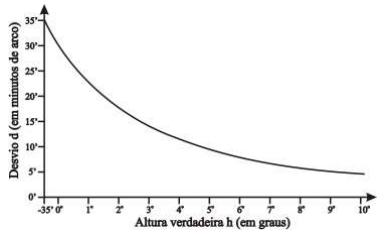
\includegraphics[scale=0.75]{img/7.png}
                \end{figure}
                \begin{itemize}
                    \item \textbf{Pergunta 7a) (0,5 ponto)} A duração do período diurno (dia claro) é afetada por este fenômeno?
                        \red{\begin{itemize}
                            \item Quando o Sol está abaixo do horizonte (se pondo ou nascendo), a refração da atmosfera o faz aparecer acima do horizonte. Portanto, esse fenômeno deixa todos os períodos maiores.
                        \end{itemize}}
                        \begin{itemize}
                            \item[$(\red{X})$] Sim, todos os periodos ficam maiores
                            \item[$(\quad)$] Sim, todos os períodos ficam menores
                            \item[$(\quad)$] Sim, os períodos ficam maiores em dias de equinócio
                            \item[$(\quad)$] Não
                        \end{itemize}
                    \item \textbf{Pergunta 7b) (0,5 ponto)} Sejam $R_b$, $R_c$, $R_d$ e $R_e$ os raios aparentes do Sol, que se encontra no horizonte, para baixo, cima, direita e esquerda respectivamente, o que podemos afirmar sobre tais medidas?
                        \red{\begin{itemize}
                            \item O fenômeno descrito só interfere na vertical, então $R_e=R_d$.
                            \item Como o deslocamento ocorre para cima, a parte inferior fica mais próxima do centro enquanto que a parte superior fica mais afastada. Portanto, $R_c>R_b$.
                        \end{itemize}}
                        \begin{itemize}
                            \item[$(\quad)$] $R_e<R_d$ e $R_c<R_b$
                            \item[$(\quad)$] $R_e>R_d$ e $R_c>R_b$
                            \item[$(\quad)$] $R_e=R_d$ e $R_c<R_b$
                            \item[$(\red{X})$] $R_e=R_d$ e $R_c>R_b$
                        \end{itemize}
                \end{itemize}
        \end{itemize} \end{flushleft}
    \section*{Questões de Astronáutica}
        \begin{flushleft} \begin{itemize}
            \item \textbf{Questão 8) (1 ponto) [OBA 2005 adaptada]} A Astronáutica é a ciência que trata da construção e operação de veículos espaciais, como os satélites e os foguetes. \linebreak \linebreak No Brasil as atividades do setor espacial são coordenadas pela Agência Espacial Brasileira (AEB), que tem a atribuição de formular e implementar o Programa Nacional de Atividades Espaciais (PNAE). O PNAE prevê a autossuficiência do Brasil na construção e lançamento de foguetes e de satélites. Além das atividades técnico-científicas, a AEB promove atividades educacionais nas escolas por meio do Programa AEB Escola, cujo objetivo é divulgar o programa espacial brasileiro e sua necessidade para o país, bem como despertar a criatividade e o gosto pela ciência entre os alunos do ensino fundamental e médio. \linebreak \linebreak Os satélites são lançados ao espaço por meio de foguetes, como os desenvolvidos pelos cientistas do Instituto de Aeronáutica e Espaço (IAE), órgão do Centro Técnico Aeroespacial (CTA). Um dos projetos em desenvolvimento no IAE é o do Veículo Lançador de Satélites, conhecido pela sigla VLS. A partir das informações coletadas pelos satélites desenvolvidos no Instituto Nacional de Pesquisas Espaciais (INPE), os cientistas brasileiros estudam o meio ambiente (clima, plantações, desmatamento das florestas, etc) em todas as regiões do país. O Instituto Tecnológico de Aeronáutica (ITA), instituição de ensino e pesquisa no setor aeroespacial, também pertence ao CTA. O CTA/IAE, o CTA/ITA e o INPE estão localizados na cidade de São José dos Campos, SP. \linebreak \linebreak Um dos centros de lançamento de foguetes brasileiros encontra-se na cidade de Alcântara, no estado do Maranhão. Trata-se do Centro de Lançamento de Alcântara (CLA). A principal vantagem deste centro é a sua localização muito próxima à linha do Equador.
                \begin{figure}[H]
                    \centering
                    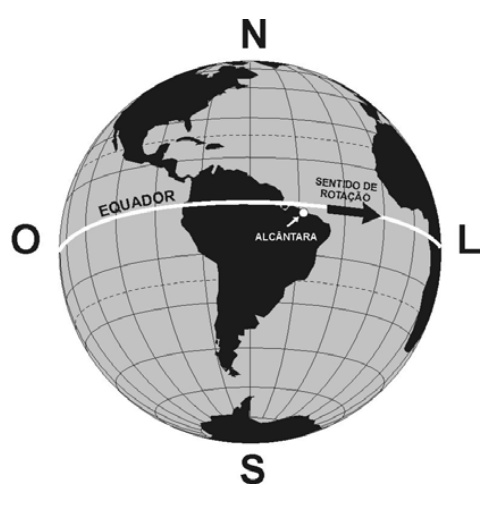
\includegraphics[scale=0.5]{img/8.png}
                \end{figure}
                \begin{itemize}
                    \item \textbf{Pergunta 8) (1 ponto)} O movimento de rotação do planeta Terra tem sentido de oeste (O) para leste (L), como indica a seta na figura acima, e será designado por O $\rightarrow$ L. Na linha do Equador esse movimento de rotação produz a maior velocidade tangencial, cujo valor é de cerca de 1.670 km/h. Para colocar um satélite em órbita a 750 km acima da superfície da Terra, o VLS deverá alcançar  a velocidade final de 28.000 km/h. Como será lançado do CLA, o VLS já partirá para o espaço com velocidade de 1.670 km/h. Com base nesses dados, qual seria o modo mais apropriado para lançar um satélite a partir de Alcântara?
                        \begin{itemize}
                            \item[$(\red{X})$] No mesmo sentido de rotação da Terra (O $\rightarrow$ L)
                            \item[$(\quad)$] No sentido contrário à rotação da Terra (L $\rightarrow$ O)
                            \item[$(\quad)$] No sentido do Pólo Norte (S $\rightarrow$ N)
                            \item[$(\quad)$] No sentido do Pólo Sul (N $\rightarrow$ S)
                        \end{itemize}
                \end{itemize}
            
            \item \textbf{Questão 9) (1 ponto) [OBA 2006 adaptada]} De acordo com o critério de que “o avião é uma máquina que pode decolar por seus próprios meios de propulsão”, Santos Dumont ficou conhecido como o inventor do avião quando o seu 14-Bis, utilizando um motor com menos de 50 HP (cavalos) de potência, voou em Bagatelle, na França, em frente a uma multidão. Tal ocorreu em 23 de outubro de 1906. Em 1971 o “Pai da Aviação”, foi proclamado “Patrono da Aeronáutica Brasileira”. A figura abaixo ilustra as forças que atuam sobre um avião. A força peso (P) é sempre vertical para baixo. A força de empuxo (E) é aquela que move o avião para a frente, sendo resultado da ação das suas turbinas que, ao consumirem o combustível, geram gases a alta velocidade. Esses gases são expelidos para trás, fazendo o avião se deslocar para frente. É o princípio da ação e reação de que trata a 3ª Lei de Newton. À medida que se desloca para a frente, aparece a força de arrasto (A), a qual resulta da interação entre o avião e a atmosfera terrestre. Essa força atua no sentido contrário ao movimento do avião. Além do arrasto, a interação do ar atmosférico com as asas do avião dá origem a uma força de sentido oposto à força peso. Trata-se da força de sustentação (S), matematicamente definida por: $$S = K \cdot \rho \cdot v^2$$ onde K é uma constante que depende da área e da orientação da asa, $\rho$ é a densidade do ar no local do voo e $v$ é a velocidade do avião em relação à atmosfera.
                \begin{figure}[H]
                    \centering
                    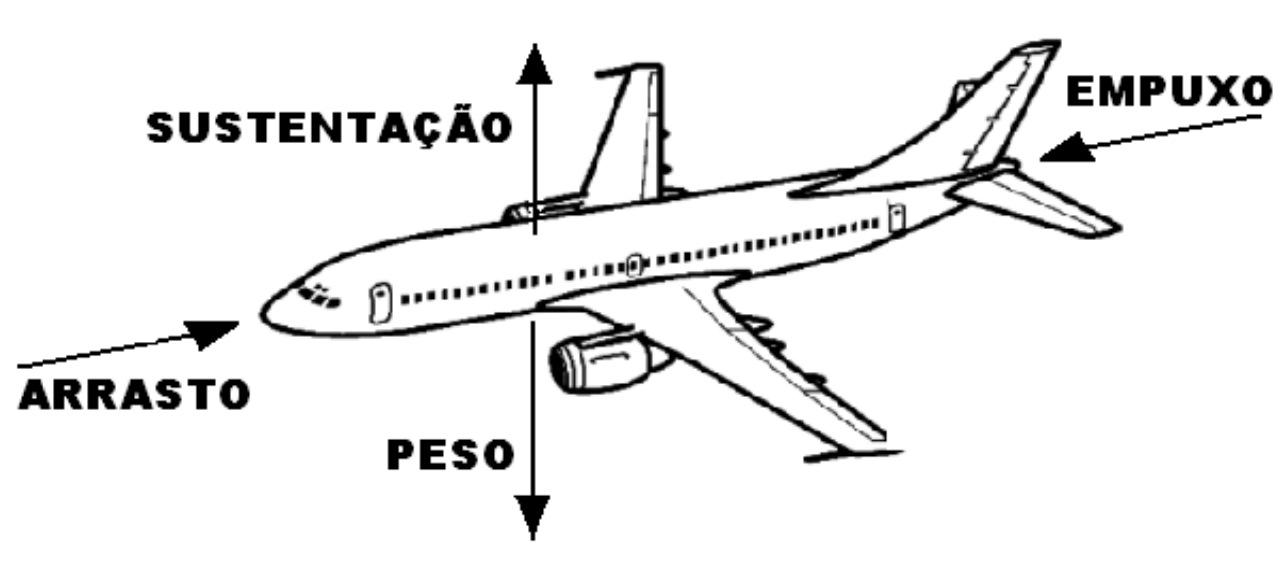
\includegraphics[scale=0.25]{img/9.png}
                \end{figure}
                \begin{itemize}
                    \item \textbf{Pergunta 9a) (0,5 ponto)} Quando o avião está parado, $S = 0$. À medida que o avião ganha velocidade, a força de sustentação aparece. Para K e $\rho$ constantes, quanto maior a velocidade, maior a força de sustentação. Se você já viu um avião decolar, você observou que ele parte do repouso, aciona suas turbinas na potência máxima e vai, gradativamente, ganhando velocidade. Existe uma velocidade na qual a força de sustentação se torna superior à força peso, $S > P$. É nesse ponto que se dá a decolagem do avião. Calcule a velocidade de decolagem do 14-Bis sabendo que sua massa (avião + piloto) era de $300 \, kg$. Para tanto, suponha: $K = 30 \, m^2$, $\rho = 1 \, \frac{kg}{m^3}$ e $g = 10 \, \frac{m}{s^2}$.
                        \red{\begin{itemize}
                            \item Quando a velocidade de decolagem é atingida, $P=S$. Portanto, temos:
                                \begin{equation*} \begin{gathered}
                                    P=S \quad \therefore \quad mg=K\rho v^2\\
                                    \therefore \quad v=\sqrt{\frac{mg}{K \rho}}=\sqrt{\frac{300 \cdot 10}{30 \cdot 1}} = 10 \, \frac{m}{s}
                                \end{gathered} \end{equation*}
                        \end{itemize}}
                        \begin{itemize}
                            \item[$(\red{X})$] $10 \, \frac{m}{s}$
                            \item[$(\quad)$] $20 \, \frac{m}{s}$
                            \item[$(\quad)$] $5 \, \frac{m}{s}$
                            \item[$(\quad)$] $25 \, \frac{m}{s}$
                        \end{itemize}
                    \item \textbf{Pergunta 9b) (0,5 ponto)} Calcule a massa do avião militar Tucano, fabricado pela Embraer, sabendo que $K = 10 m^2$ e que ele decola com velocidade $v = 180 \frac{km}{h}$. Suponha $\rho = 1 \frac{kg}{m^3}$ e $g = 10 \frac{m}{s^2}$.
                        \red{\begin{itemize}
                            \item Primeiramente, precisamos converter as unidades da velocidade informada:
                                \begin{equation*}
                                    v=\frac{180}{3,6}=50 \, \frac{m}{s}
                                \end{equation*}
                            \item Agora, basta usarmos a mesma estratégia da pergunta anterior para encontrar a massa:
                                \begin{equation*} \begin{gathered}
                                    P=S \quad \therefore \quad mg=K\rho v^2\\
                                    \therefore \quad m=\frac{K\rho v^2}{g}=\frac{10 \cdot 1 \cdot 50^2}{10}= 2.500 \, kg
                                \end{gathered} \end{equation*}
                        \end{itemize}}
                        \begin{itemize}
                            \item[$(\red{X})$] $2.500 \, kg$
                            \item[$(\quad)$] $250 \, kg$
                            \item[$(\quad)$] $5.000 \, kg$
                            \item[$(\quad)$] $500 \, kg$
                        \end{itemize}
                \end{itemize}

            \item \textbf{Questão 10) (1 ponto) [OBA 2006 adaptada]} O movimento que os veículos espaciais descrevem em torno da Terra é governado pelas mesmas leis que regem o movimento dos planetas em torno do Sol. As bases dessas leis foram descobertas por alguns dos mais importantes cientistas que já existiram. Isaac Newton (1642-1727) formulou a Lei da Gravitação Universal, segundo a qual a força de atração entre dois corpos é diretamente proporcional às suas massas e inversamente proporcional ao quadrado da distância que os separam. Para formular essa lei ele se baseou em três importantes leis da mecânica celeste, que foram anteriormente formuladas pelo astrônomo Kepler (1571-1630). Kepler, por sua vez, formulou suas leis para explicar as observações feitas por Tycho Brahe (1546-1601), astrônomo que fez o maior catálogo de observações dos astros celestes da época. As três leis de Kepler são enunciadas da seguinte forma: \linebreak \linebreak 1) Todo planeta descreve órbita elíptica ao redor do Sol, estando este num dos focos da elipse. \linebreak 2) A linha que une o planeta ao Sol varre áreas iguais em iguais intervalos de tempo. \linebreak 3) A razão entre o quadrado do período da órbita e o cubo da distância entre os centros dos corpos envolvidos é uma constante. \linebreak \linebreak Com base na terceira Lei de Kepler, é possível relacionar o período de uma órbita circular com o seu raio. Ou seja, é possível relacionar o tempo que leva para o planeta dar uma volta em torno do Sol com a distância entre os centros do Sol e do planeta. Aplicando essa mesma lei para a órbita da Estação Espacial Internacional (ISS) em torno da Terra, é possível construir a tabela mostrada abaixo, que relaciona o período orbital com o raio de uma órbita circular. \linebreak \linebreak A ISS gira em torno da Terra numa órbita circular de raio igual a 6.727 km, ou seja, a 350 km acima da superfície terrestre. Esse dado foi utilizado para a programação da missão espacial para a qual foi escalado o primeiro astronauta brasileiro a ir ao espaço. Marcos Pontes foi lançado ao espaço a bordo de uma nave russa em 29 de março de 2006. De acordo com a missão, ele entrou a bordo da ISS às 04 horas e 13 minutos (horário de Greenwich) do dia 1 de abril de 2006, e permaneceu na ISS até às 17 horas e 12 minutos do dia 8 de abril de 2006 (também horário de Greenwich). Com base nesses dados, calcule e responda às questões abaixo.
                \begin{figure}[H]
                    \centering
                    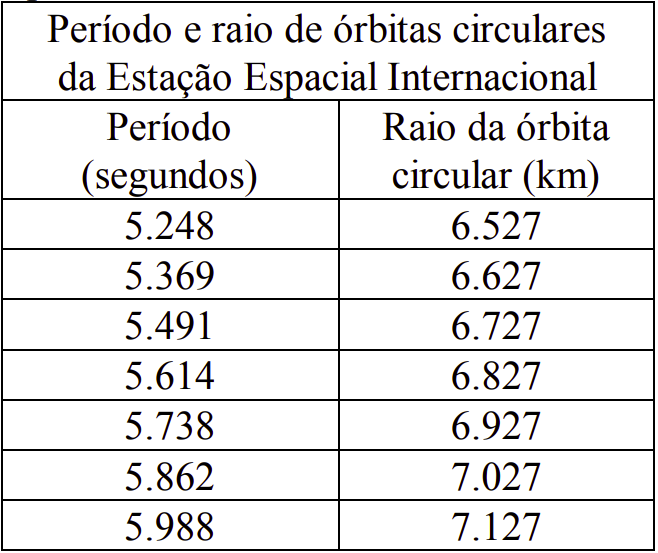
\includegraphics[scale=0.35]{img/10.png}
                \end{figure}
                \begin{itemize}
                    \item \textbf{Pergunta 10a) (0,25 ponto)}  Quantas horas e minutos o astronauta brasileiro Pontes permaneceu no espaço a bordo da ISS?
                        \red{\begin{itemize}
                            \item Para evitar um erro de cálculo, podemos dividir a permanência do astronauta na ISS em 3 intervalos. O primeiro é de sua chegada até o próximo dia:
                                \begin{equation*}
                                    \Delta t_1=24h - 4h \, 13min=19h \, 47min
                                \end{equation*}
                            \item O segundo intervalo é de seu segundo dia (2 de abril) até seu penúltimo dia (7 de abril):
                                \begin{equation*}
                                    \Delta t_2=6 \cdot 24h=144h
                                \end{equation*}
                            \item O terceiro intervalo é a sua permanência durante seu último dia:
                                \begin{equation*}
                                    \Delta t_3=17h \, 12min
                                \end{equation*}
                            \item Somando tudo, temos:
                                \begin{equation*}
                                    \Delta t=\Delta t_1 + \Delta t_2+\Delta t_3=180h \, 59min
                                \end{equation*}
                        \end{itemize}}
                        \begin{itemize}
                            \item[$(\red{X})$] $180h \, 59min$
                            \item[$(\quad)$] $156h \, 59min$
                            \item[$(\quad)$] $36h \, 59min$
                            \item[$(\quad)$] $165h \, 25min$
                        \end{itemize}
                    \item \textbf{Pergunta 10b) (0,25 ponto)} Qual é o período orbital da ISS, em horas e minutos, quando o raio da sua órbita é aquele dado no parágrafo acima?
                        \red{\begin{itemize}
                            \item Analisando a tabela dada, temos o período em segundos:
                                \begin{equation*}
                                    T=5.491 \, s
                                \end{equation*}
                            \item Convertendo esse valor para as unidades pedidas, temos:
                                \begin{equation*}
                                    T=1h \, 31min \, 31s \approx 1h \, 32min
                                \end{equation*}
                        \end{itemize}}
                        \begin{itemize}
                            \item[$(\red{X})$] $1h \, 32min$
                            \item[$(\quad)$] $1h \, 27min$
                            \item[$(\quad)$] $1h \, 40min$
                            \item[$(\quad)$] $1h \, 22min$
                        \end{itemize}
                    \item \textbf{Pergunta 10c) (0,5 ponto)} Quantas voltas o astronauta brasileiro deu em torno da Terra ao completar sua missão a bordo da ISS?
                        \red{\begin{itemize}
                            \item Basta dividir os valores calculados nas perguntas anteriores:
                                \begin{equation*}
                                    N=\frac{\Delta t}{T}=\frac{180h \, 59min}{1h \, 32min} \approx 118
                                \end{equation*}
                        \end{itemize}}
                        \begin{itemize}
                            \item[$(\red{X})$] $118$
                            \item[$(\quad)$] $102$
                            \item[$(\quad)$] $125$
                            \item[$(\quad)$] $89$
                        \end{itemize}
                \end{itemize}
        \end{itemize} \end{flushleft}
    \section*{Questões avançadas}
        \begin{flushleft} \begin{itemize}
            \item \textbf{Questão 11) (1 ponto)} Deneb é uma estrela de tipo espectral A2 cuja magnitude aparente na banda V é de 1,25. Certa noite Deneb se divide em 2 novas estrelas com a mesma temperatura da inicial. \linebreak \linebreak Dado: \linebreak $\log(2) \approx 0,3$
                \begin{itemize}
                    \item \textbf{Pergunta 11) (1 ponto)} Qual a nova magnitude aparente na banda V do sistema?
                        \red{\begin{itemize}
                            \item Como o volume de cada uma das novas estrelas deve ser metade de Deneb, temos a seguinte relação entre os raios das novas estrelas ($R'$) e de Deneb ($R_0$):
                                \begin{equation*}
                                    V'=\frac{V_0}{2} \quad \therefore \quad \frac{4\pi R'^3}{3}=\frac{1}{2} \frac{4 \pi R_0^3}{3} \quad \therefore \quad \frac{R'}{R_0}=\sqrt[3]{\frac{1}{2}}
                                \end{equation*}
                            \item Lembrando que $T'=T_0$, podemos usar a equação de Stefan-Boltzmann para encontrar a razão entre as luminosidades:
                                \begin{equation*}
                                    \frac{L'}{L_0}=\frac{4 \pi R'^2 \sigma T'^4}{4 \pi R_0^2 \sigma T_0^4}=\left(\frac{R'}{R_0}\right)^2=2^{-\frac{2}{3}}
                                \end{equation*}
                            \item Calculando a razão dos fluxos recebidos, temos:
                                \begin{equation*}
                                    \frac{F'}{F_0}=\frac{2L'}{L_0}=2 \cdot 2^{-\frac{2}{3}}=\sqrt[3]{2}
                                \end{equation*}
                            \item Finalmente, usando a relação de Pógson, temos:
                                \begin{equation*} \begin{gathered}
                                    m'-m_0=2,5 \log \left(\frac{F_0}{F'}\right) \quad \therefore \quad m'=2,5 \log \left(\frac{F_0}{F'}\right)+m_0\\
                                    \therefore \quad m'=2,5 \log \left(2^{-\frac{1}{3}}\right)+1,25=-\frac{2,5 \cdot \log (2)}{3}+1,25\\
                                    \therefore \quad m'=-0,25 +1,25 =1,0
                                \end{gathered} \end{equation*}
                        \end{itemize}}
                        \begin{itemize}
                            \item[$(\quad)$] $1,25$
                            \item[$(\quad)$] $2,5$
                            \item[$(\red{X})$] $1,0$
                            \item[$(\quad)$] $2,0$
                        \end{itemize}
                \end{itemize}
            
            \item \textbf{Questão 12) (1 ponto)} Relógios de Sol são usados há muito tempo para determinar a hora em diversos locais do mundo. A ideia deste tipo de relógio é utilizar o ângulo horário do Sol para atingir o objetivo. Esse método, no entanto, tem um grande problema, que é o fato do Sol não se comportar da mesma maneira todos os dias, levando ao mesmo ângulo horário representar horários diferentes para dias diferentes. Para que consigamos descobrir com precisão a hora para um dado dia utilizamos a Equação do Tempo, que gera uma correção numérica à medição, levando-nos ao valor correto.
                \begin{itemize}
                    \item \textbf{Pergunta 12) (1 ponto)} Quais dos fatores abaixo podemos apontar como os principais que influenciam essa incongruência das medições?
                        \begin{itemize}
                            \item[$(\red{X})$] A excentricidade não nula da órbita da Terra
                            \item[$(\red{X})$] A obliquidade do eixo de rotação da Terra
                            \item[$(\quad)$] A rotação do Sol
                            \item[$(\quad)$] O formato da Terra
                        \end{itemize}
                \end{itemize}
            
            \item \textbf{Questão 13) (1 ponto)} Um fenômeno muito conhecido é o da ``laçada de Marte", em que o planeta Marte subitamente muda sua direção de deslocamento no céu, e quando acompanhado por vários dias parece se locomover formando um laço no céu.
                \begin{itemize}
                    \item \textbf{Pergunta 13) (1 ponto)} Quais planetas, além de Marte, reproduzem o mesmo fenômeno de modo que possamos observá-los em uma noite de céu limpo?
                        \red{\begin{itemize}
                            \item Todos os planetas reproduzem esse fenômeno. Então, a pegadinha da questão é você marcar somente os planetas que são observáveis à noite, excluindo assim os planetas inferiores (Mercúrio e Vênus), os quais estão sempre próximos ao Sol na Esfera Celeste.
                        \end{itemize}}
                        \begin{itemize}
                            \item[$(\quad)$] Mercúrio
                            \item[$(\quad)$] Vênus
                            \item[$(\red{X})$] Júpiter
                            \item[$(\red{X})$] Saturno
                            \item[$(\red{X})$] Urano
                            \item[$(\red{X})$] Netuno
                        \end{itemize}
                \end{itemize}

            \item \textbf{Questão 14) (1 ponto)}
                \begin{itemize}
                    \item \textbf{Pergunta 14) (1 ponto)} Vamos considerar a existência de 2 cometas que orbitam o Sol; o cometa A possui uma órbita de excentricidade 0,87 e o B uma órbita de excentricidade 1,5. Ambos foram observados no dia 5 de março de 2020 por um observador na Terra. Eles poderão ser avistados novamente pelo observador? Considere que este dia foi o único no qual os cometas puderam ser avistados no mês de março e ambos apresentavam magnitude 6.
                        \red{\begin{itemize}
                            \item Órbitas com excentricidade $e < 1$ são elípticas, possuindo assim uma periodicidade. Já órbitas com excentricidade $e > 1$ são hiperbólicas, não possuindo uma periodicidade. Portanto, somente o cometa A poderá ser visto novamente.
                        \end{itemize}}
                        \begin{itemize}
                            \item[$(\red{X})$] Apenas o A poderá ser visto novamente
                            \item[$(\quad)$] Apenas o B poderá ser visto novamente
                            \item[$(\quad)$] Ambos poderão ser vistos novamente
                            \item[$(\quad)$] Nenhum dos 2 poderá ser visto novamente
                        \end{itemize}
                \end{itemize}
        \end{itemize} \end{flushleft}
\end{document}